\documentclass[a4paper,12pt]{article}

%%%%%%%%%%%%%%%%%%%%
%%%%  PREAMBLE  %%%%
%%%%%%%%%%%%%%%%%%%%

\usepackage[T1]{fontenc}
\usepackage[utf8]{inputenc}

\usepackage[english,italian]{babel}

\usepackage{hyperref}
\hypersetup{hidelinks}

\usepackage[margin=2.5cm]{geometry}
\usepackage{minipage-marginpar}
\usepackage{fancyhdr}
\usepackage[bottom]{footmisc}
\usepackage{lastpage}

\usepackage{enumitem}

\usepackage{graphicx}

\setlength{\parindent}{0em}
\setlength{\parskip}{1em}

\fancyhead[L]{\leftmark}
\fancyhead[R]{\shortstack[r]{Versione documento: 0.03 \\ Gruppo: T27}}

\fancyfoot[C]{}
\fancyfoot[R]{\thepage/\pageref{LastPage}}

\renewcommand{\headrulewidth}{2pt}
\renewcommand{\headruleskip}{3pt}
\setlength{\headheight}{30pt}

\renewcommand{\footrulewidth}{2pt}

\setlist[itemize]{itemsep=0.25em,topsep=0pt}
\setlist[enumerate]{itemsep=0.75em,topsep=0pt,align=left}

%%%%%%%%%%%%%%%%%%%%
%%%%  DOCUMENT  %%%%
%%%%%%%%%%%%%%%%%%%%

\title{Web Music Player}
\author{Gruppo T27}

\begin{document}

\pagestyle{empty}

\begin{center}

    \vspace{2 cm}

    \begin{tabular*}{\textwidth}{ c @{\extracolsep{\fill}} c }
        
\includegraphics[width=0.3\textwidth]{marchio_unitrento.pdf} & \shortstack{\Large{Dipartimento di Ingegneria} \\ \Large{e Scienza dell'Informazione}}
    \end{tabular*}

    \vspace{2 cm} 
  
    \LARGE{Ingegneria del software\\}
  
    \vspace{1.5 cm} 
    \Large\textsc{Documento di progetto\\} 
    \Large\textsc{Versione: 0.03\\} 
    \vspace{2 cm} 
    \Huge\textsc{Web Music Player\\}
    \Large{\it{Gruppo T27}}
  
    \vspace{2 cm} 
  
    \Large{Anno accademico 2022/2023}
\end{center}

\newpage
\tableofcontents

\pagestyle{fancy}

\newpage
\section{Scopo del documento}

Il presente documento riporta l’analisi dei requisiti di sistema del progetto Web Music Player in linguaggio naturale. Lo scopo di questo di questo documento è quello di:
\begin{itemize}
    \item descrivere gli obiettivi del progetto;
    \item elencare i requisiti funzionali;
    \item elencare i requisiti non funzionali;
    \item presentare il front-end del progetto;
    \item descrivere il back-end del progetto.
\end{itemize}

\section{Obiettivi del progetto}

Il progetto ha come obiettivo la realizzazione di una piattaforma online per l’ascolto di musica. Questo servizio deve offrire le funzionalità di un moderna piattaforma di streaming, focalizzandosi sull’utente e in particolare sulla proposta di nuova musica basata sui contenuti ascoltati.

Nello specifico, il servizio deve essere in grado di:

\begin{itemize}
    \item dare la possibilità ad un nuovo utente di registrarsi al suo primo accesso al sito web. Per la registrazione sono necessari un indirizzo email e una password. Un utente già registrato deve avere la possibilità di effettuare l’accesso tramite le sue credenziali;
    \item permettere a chi produce musica di registrarsi come creator. Questi utenti possono caricare la propria musica sulla piattaforma attraverso una schermata apposita nel loro profilo. Possono essere caricate gruppi di canzoni racchiuse in album, mixtape, EP;
    \item un utente dev’essere in grado di cercare, ascoltare e riprodurre musica in streaming. Ha la possibilità di aggiungere alla Libreria canzoni, album e creare nuove playlist;
    \item suggerire nuova musica sulla base dei gusti dell’utente. Questi vengono determinati dalle canzoni ascoltate, dai loro tag, dalle playlist create e dagli album salvati. L’utente deve essere in grado di interagire con le proposte, approvando i nuovi suggerimenti o rifiutandoli. In entrambi i casi, le decisioni vengono prese in considerazione per le future proposte.
\end{itemize}

\newpage
\section{Requisiti funzionali}

Presentiamo ora i requisiti funzionali del sistema: le funzionalità offerte dal nostro servizio.

\begin{enumerate}[label=\textbf{RF\arabic*}\;, ref=\textbf{RF\arabic*}]
    \item \label{registrazione} \textbf{Registrazione}
    
    Il software deve presentare una schermata di registrazione agli utenti che visitano per la prima volta il sito. Sono presenti due modalità di registrazione: utente standard e utente creator. Per registrarsi, in entrambe le modalità, sono necessari un indirizzo email valido ed una password sicura (vedi \ref{password sicura}). Per completare la fase di registrazione l'indirizzo email non deve essere associato ad un account esistente, e dev'essere verificato (vedi \ref{email di verifica}). Una volta fatto ciò, si passa alla fase di pagamento.
    \item \label{pagamento} \textbf{Pagamento}

    Una volta completata la registrazione, il software deve portare una schermata per il pagamento (vedi \ref{pagamento non funzionale}). Gli utenti potranno pagare secondo due modalità: pagamento con la carta di credito o tramite PayPal. Una volta confermato il pagamento, si potrà accedere al servizio tramite login.
    \item \label{login} \textbf{Login}
    
    Il software deve fornire una schermata di login nella quale gli utenti registrati possono inserire email e password per accedere.
    \item \label{recupero password} \textbf{Recupero password}

    Dalla schermata di accesso è possibile accedere tramite testo cliccabile al recupero password (vedi \ref{recupero password nf}).
    \item \label{ricerca} \textbf{Ricerca}
    
    Gli utenti possono cercare releases\footnote{Release: contenuto musicale caricato da un creator; ciò include singoli, album, EP, mixtapes.} o playlist create tramite una barra di ricerca. Possono effettuare le ricerche tramite i metadati dei brani. Si possono ricercare gli artisti tramite il nome.
    \item \label{riproduzione} \textbf{Riproduzione}
    
    Gli utenti possono riprodurre una release o una playlist selezionata; un brano in riproduzione può essere messo in pausa.
    \item \label{coda} \textbf{Coda}

    Quando un brano viene riprodotto, vengono messi in coda\footnote{Coda: lista di canzoni riprodotte automaticamente quando quella corrente termina.} eventuali canzoni ad essa legate, ovvero le canzoni successive nel caso in cui la canzone faccia parte di una playlist o di una release, fino alla fine. Gli utenti possono passare alla canzone successiva o alla precedente tramite pulsanti appositi (sequenzialità) oppure riprodurre la coda in ordine casuale.
    \item \label{libreria} \textbf{Libreria}

    Il software deve offrire una sezione chiamata Libreria per raggruppare la musica salvata dall’utente (vedi \ref{preferiti}) e le playlist create.

    \item \label{preferiti} \textbf{Preferiti}
    
    Il software deve permettere all’utente di salvare releases nella libreria in una zona “Preferiti".
    \item \label{playlist} \textbf{Playlist}
    
    Il software deve permettere all’utente di creare e gestire (spostare, rimuovere) le proprie playlist nella Libreria.
    \item \label{consigliati} \textbf{Consigliati}
    
    Il software deve suggerire all’utente altre releases basandosi principalmente sugli ascolti passati, sui tag di quel brani, sulle playlist create e sugli album salvati.
    \item \label{feedback} \textbf{Feedback}
    
    L’utente deve poter dare un’opinione del brano consigliato dal sistema.
    \item \label{cronologia} \textbf{Cronologia}
    
    Il software deve mostrare release e playlist ascoltate in ordine cronologico inverso (dal più recente al meno recente), fino a un massimo di 30 brani.
    \item \label{impostazioni} \textbf{Impostazioni}
    
    Dalla schermata principale sarà possibile aprire la schermata impostazioni. Da qui sarà possibile effettuare il logout (vedi \ref{logout}), disdire l'abbonamento (vedi \ref{disdire l'abbonamento}), cambiare la password (vedi \ref{cambiare password}), cambiare la lingua di visualizzazione (vedi \ref{lingue}) ed eliminare l'account (vedi \ref{cancellazione account}).
    \item \label{logout} \textbf{Effettuare il log-out}
    
    L'utente può effettuare il log-out dal proprio account dalla pagina delle impostazioni. La disconnessione porterà l'utente alla schermata di login, dalla quale sarà necessario effettuare l'accesso per poter tornare ad utilizzare il servizio.
    \item \label{cancellazione account} \textbf{Cancellazione account}
    
    L'utente può richiedere la rimozione del suo account dalla pagina delle impostazioni. Viene chiesto di confermare la scelta, e in caso di risposta affermativa le informazioni dell'utente saranno rimosse completamente dalla piattaforma.
    \item \label{disdire l'abbonamento} \textbf{Disdire l'abbonamento}
    
    L'utente può disdire l'abbonamento corrente dalla pagina delle impostazioni. Viene chiesto di confermare la scelta e se l’utente conferma, il servizio sarà disponibile fino al termine del mese per il quale ha pagato.
    \item \label{lingue} \textbf{Cambiare lingua}
    
    L'utente può cambiare la lingua della piattaforma dalla schermata delle impostazioni. È possibile scegliere tra le lingue disponibili al momento della scelta.
    \item \label{account creator} \textbf{Account creator}
    
    Gli utenti creator possono usufruire di tutti i servizi dell’account standard. Possono inoltre accedere ad una schermata relativa al proprio account (vedi \ref{visualizzare account creator}) dove possono caricare le proprie releases (vedi \ref{caricamento release}), modificare quelle già presenti (vedi \ref{modifica release}) o eliminarle dalla piattaforma (vedi \ref{eliminazione release}).
    \item \label{visualizzare account creator} \textbf{Visualizzare account creator}
    
    Gli utenti standard e creator possono visualizzare il profilo di un artista per vedere tutte le sue releases.
    \item \label{caricamento release} \textbf{Carimento releases}
    
    Gli utenti creator possono caricare nuova musica sulla piattaforma dalla schermata relativa al proprio account. Il creator dovrà scegliere la release da caricare, avverrà il caricamento sulla piattaforma, dove sarà visualizzata nell’apposito elenco, quindi dei singoli o degli album.
    \item \label{modifica release} \textbf{Modifica release}
    
    Gli utenti creator possono modificare le releases pubblicate sulla piattaforma dalla schermata relativa al proprio account. Possono modificarne il titolo e i tag assegnati. 
    \item \label{eliminazione release} \textbf{Eliminazione release}
    
    Gli utenti creator possono eliminare delle releases da loro pubblicate sulla piattaforma. Possono fare ciò dalla schermata relativa al proprio account.
\end{enumerate}

\newpage
\section{Requisiti non funzionali}

Presentiamo i requisiti non funzionali del sistema: le proprietà globali del nostro servizio.

\begin{enumerate}[label=\textbf{RNF\arabic*}\;, ref=\textbf{RNF\arabic*}]
    \item \label{portabilità} \textbf{Portabilità}
    
    Il servizio deve essere accessibile dai browser di computer fissi e portatili. Deve supportare i principali browser in commercio: Safari, Edge, Firefox e Chrome; supportare le versioni rilasciate entro il 2017.
    \item \label{security} \textbf{Security}
    
    \begin{enumerate}[label=\textbf{\alph*}, ref=\textbf{RNF2\alph*}, itemsep=0.5em]
        \item \label{password sicura} per password “sicura” si intende: lunghezza di almeno 8 caratteri, almeno una lettera maiuscola e minuscola, almeno un numero, almeno un carattere speciale (\%\&\#!@*\^\,);
        \item \label{email di verifica} alla registrazione il software invia una mail all’indirizzo inserito dall’utente contenente un link da cliccare. Una volta cliccato il link, la mail viene validata e l’account è registrato. Questo per garantire che l’indirizzo email esista ed appartenga all’utente;
        \item \label{protocollo https} utilizzo del protocollo https per una connessione cifrata;
        \item \label{DRM} quanto più streaming di risorse protette da diritto di copyright possibile dev’essere protetto attraverso un sistema DRM per la protezione di tali diritti, in modo da evitare per quanto possibile la diffusione non autorizzata delle suddette risorse.
    \end{enumerate}
    \item \label{recupero password nf} \textbf{Recupero password}
    
    Il software offre la possibilità di recuperare la password attraverso l’indirizzo email associato all’account.
    \item \label{cambiare password} \textbf{Cambiare la password}
    
    L'utente ha la possibilità di cambiare la password associata al suo account.
    \item \label{affidabilità} \textbf{Affidabilità}
    
    L’infrastruttura è ridondata per garantire la protezione dal fallimento di dischi. Il servizio deve eseguire un backup dei dati mensilmente. Questi backup sono salvati su un servizio esterno, in modo da assicurare la conservazione dei dati in caso di guasti all’infrastruttura o di attacco hacker.
    \item \label{usabilità} \textbf{Usabilità}
    
    L’applicazione deve risultare familiare per un target di giovani e giovani adulti di età compresa tra i 16 e 35 anni, previa esperienza nell’utilizzo di un contemporaneo dispositivo digitale (dal 2015 in poi).
    \item \label{privacy} \textbf{Privacy}
    
    Conforme alle norme esposte nel GDPR.
    \item \label{performance} \textbf{Performance}
    
    \begin{enumerate}[label=\textbf{\alph*}, ref=\textbf{RNF6\alph*}, itemsep=0.5em]
        \item \label{qualità streaming} lo streaming deve adattarsi alla banda disponibile all’utente in quel momento, diminuendo o aumentando la qualità, in base allo stato della rete;
        \item \label{velocità ricerca} la ricerca nella barra di ricerca deve restituire risultati entro 10 secondi con una media di 3 secondi.
    \end{enumerate}

    \item \label{pagamento non funzionale} \textbf{Pagamento}
    
    L’abbonamento viene fatturato mensilmente.
    \item \label{tag} \textbf{Tag}
    
    I tag che vengono assegnati automaticamente alle releases provengono dall’autore e da servizi esterni (last.fm, musicbrainz).
\end{enumerate}

\section{Front-end}

Descriviamo il software dal punto di vista dell'interfaccia.

\begin{enumerate}[label=\textbf{FE\arabic*}\;, ref=\textbf{FE\arabic*}]
    \item \label{schermata registrazione} \textbf{Schermata registrazione}
    
    L'interfaccia presenta dei campi testuali per inserire email, password e conferma password. Presenta due bottoni per scegliere il tipo di account e un bottone per registrarsi.

    \begin{figure}[ht]
        \centering
        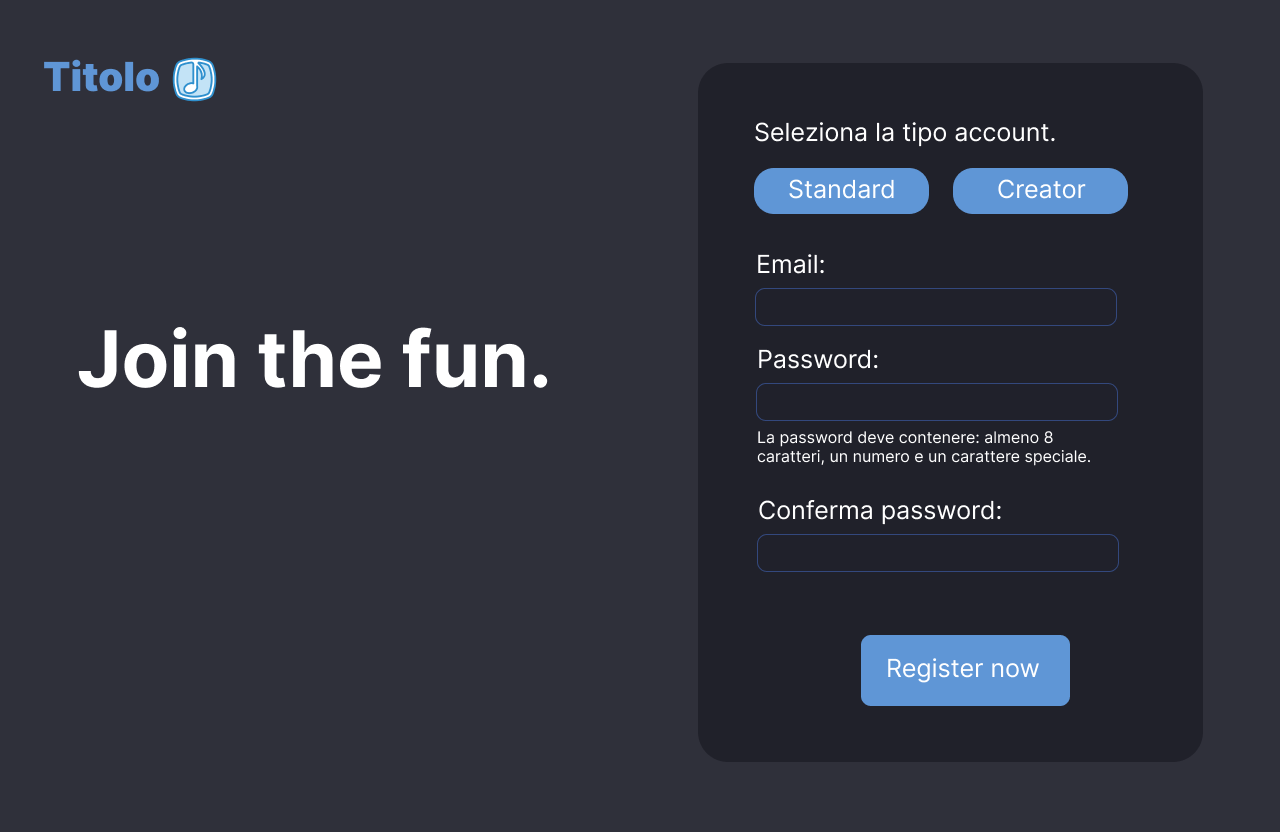
\includegraphics[width=0.8\textwidth]{schermata registrazione.png}
        \caption{Schermata registrazione}
        \label{fig:schermata_registrazione}
    \end{figure}

    \item \label{schermata pagamento} \textbf{Schermata pagamento}
    
    L'interfaccia presenta due bottoni per scegliere il metodo di pagamento: uno per le carte di credito, uno per PayPal.
    \item \label{schermata login} \textbf{Schermata login}
    
    L'interfaccia presenta dei campi testuali per inserire email e password. Presenta una scritta cliccabile per recuperare la password ed un bottone per effettuare l'accesso. È inoltre presente una scritta cliccabile per passare alla pagina della registrazione.

    \begin{figure}[ht]
        \centering
        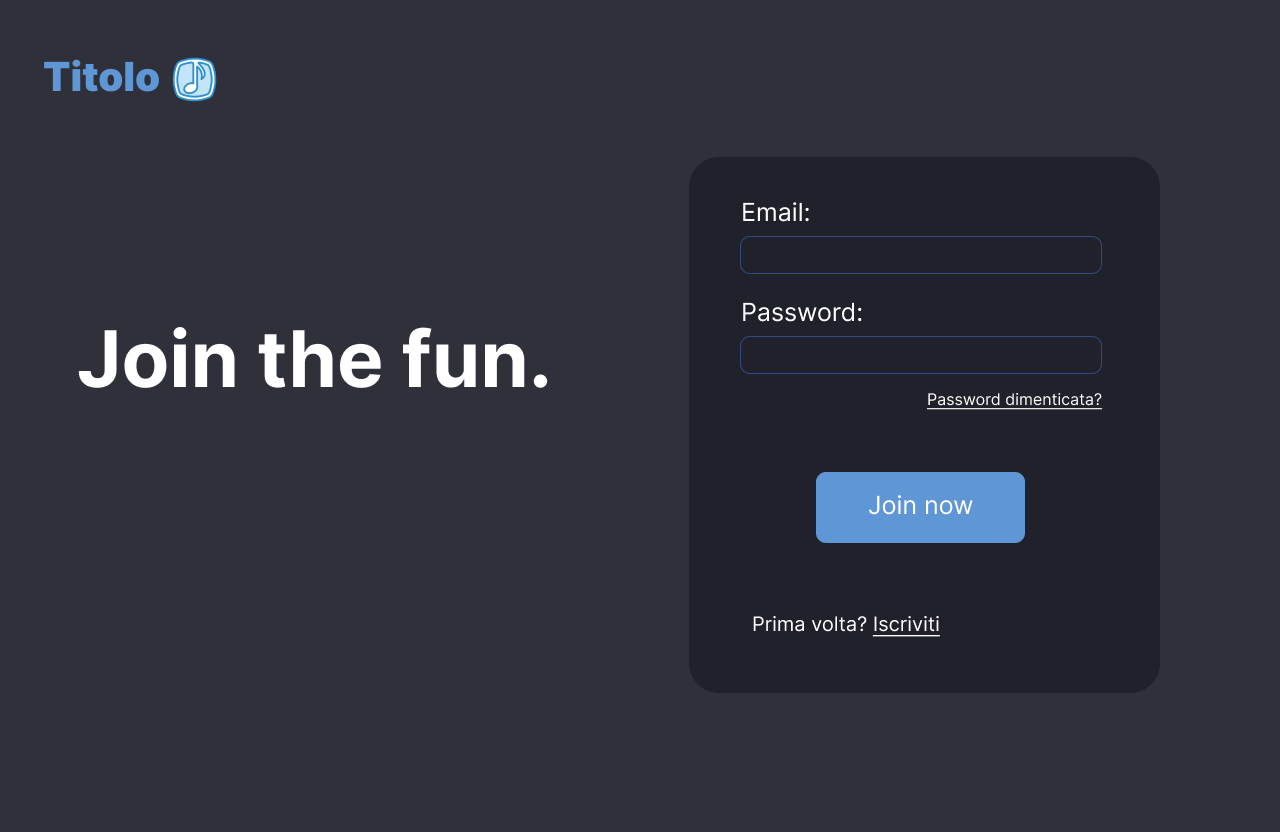
\includegraphics[width=0.8\textwidth]{schermata login.png}
        \caption{Schermata login}
        \label{fig:schermata_login}
    \end{figure}

    \item \label{schermata recupero password} \textbf{Schermate recupero password}
    
    Vedi \ref{recupero password nf}. La prima schermata presenta una componente testuale per inserire la mail alla quale inviare il link. La seconda schermata presenta due aree testuali per inserire e confermare la nuova password.
    \item \label{barra superiore} \textbf{Schermata principale: barra superiore}
    
    Composta da: logo a sinistra, barra di ricerca (\ref{ricerca}) al centro e il bottone per le impostazioni a destra. 
    \item \label{scheda a sinistra} \textbf{Schermata principale: scheda a sinistra}
    
    Schermata che suggerisce i brani (\ref{consigliati}): titolo della scheda seguito da una lista di brani. Ogni brano presenta a lato due pulsanti: una X per dire che il brano non è stato apprezzato e un cuore per indicare che gli piace.
    \item \label{scheda centrale} \textbf{Schermata principale: scheda centrale}
    
    Leggermente più grande delle altre. Schermata libreria (\ref{libreria}). Al suo interno sono presenti 2 sottosezioni: la prima presenta i preferiti (\ref{preferiti}), la seconda playlist create (\ref{playlist}). Cliccando sul titolo di una delle sottosezioni la tab libreria verrà sostituita da questa sottosezione. Nella nuova vista troviamo in alto a sinistra un bottone per tornare indietro, seguito dal titolo della sottosezione. Sotto, l’elenco delle releases salvate o delle playlist. Cliccare sul nome di una playlist o una release che non sia un singolo aprirà sulla tab centrale una vista di quella playlist/album/ep/mixtape, con in alto un bottone per tornare indietro e il titolo, subito sotto l'elenco dei brani.
    \item \label{scheda a destra} \textbf{Schermata principale: scheda a destra}
    
    La cronologia di ascolto. Vedi \ref{cronologia}.
    \item \label{barra inferiore} \textbf{Schermata principale: barra inferiore}
    
    Presenta a sinistra titolo e l’artista della canzone che si sta ascoltando, al centro: 3 pulsanti: canzone precedente, successiva, play-pause.

    \begin{figure}[ht]
        \centering
        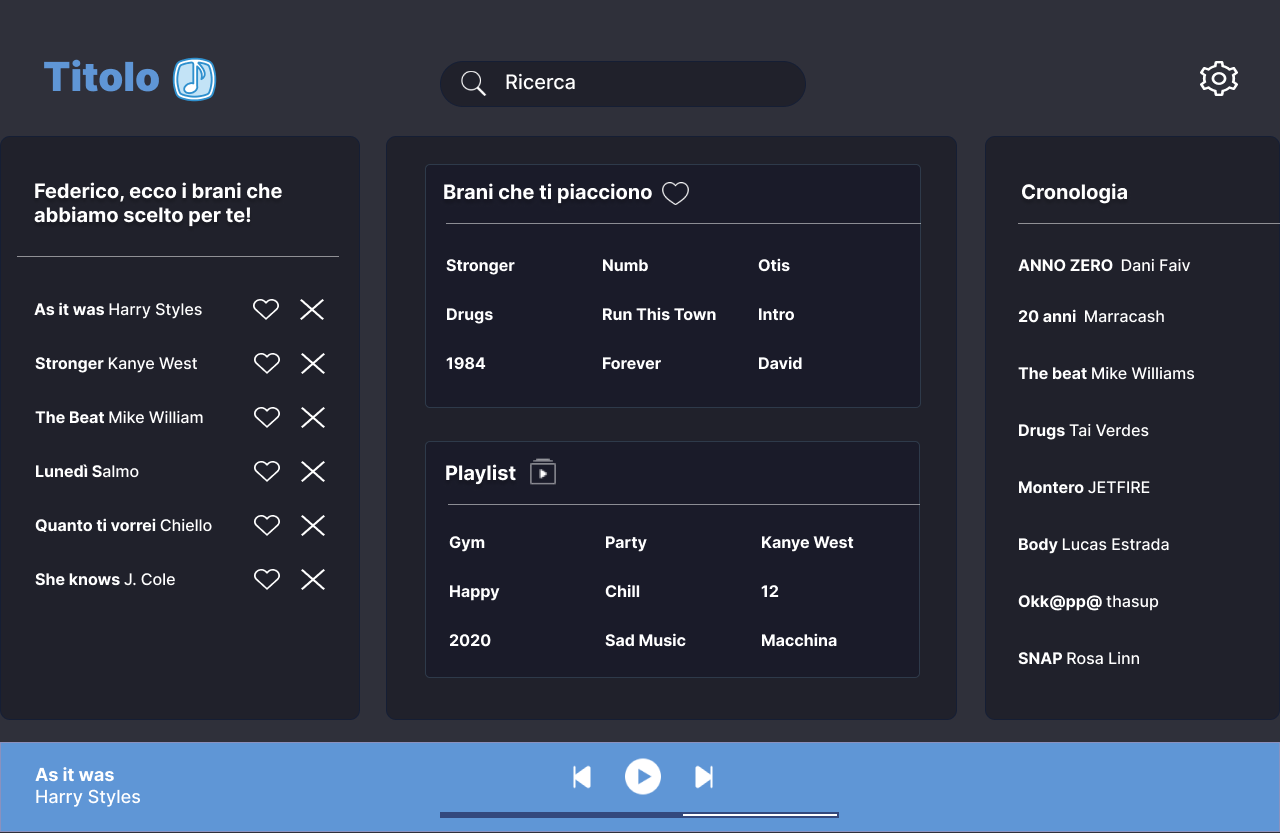
\includegraphics[width=0.8\textwidth]{schermata principale.png}
        \caption{Schermata principale}
        \label{fig:schermata_principale}
    \end{figure}

    \item \label{schermata impostazioni} \textbf{Schermata impostazioni}
    
    Elenco di opzioni nel formato “Descrizione - Bottone acceso/spento” oppure “Descrizione - Menù a tendina”. Vedi \ref{impostazioni}.
    \item \label{schermata account creator} \textbf{Schermata account creator}
    
    La schermata presenta il nome del creator in alto a destra e un bottone per tornare indietro in alto a sinistra. Al centro presenta due elenchi: i singoli caricati e gli album caricati.

    \begin{figure}[ht]
        \centering
        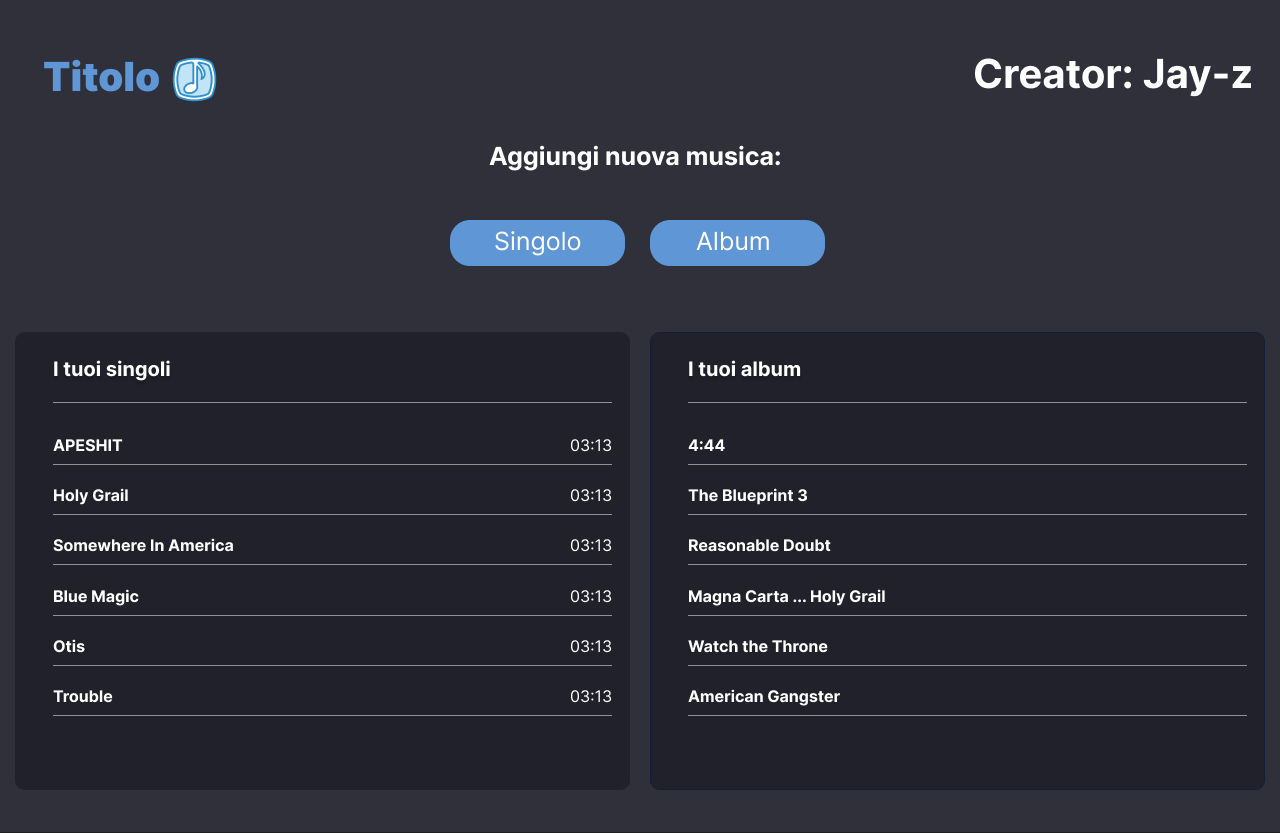
\includegraphics[width=0.8\textwidth]{schermata creator.png}
        \caption{Schermata creator}
        \label{fig:schermata_creator}
    \end{figure}

    \item \label{creazione playlist} \textbf{Creazione playlist}
    
    Quando un brano va aggiunto ad una playlist, appare una schermata nella quale sono elencate le playlist esistenti, e tramite pulsante si potrà creare una nuova playlist ed inserire il nome. Vedi \ref{playlist}. 
\end{enumerate}

\section{Back-end}

Descriviamo il software dal punto di vista dei sistemi con il quale deve interagire.

\begin{enumerate}[label=\textbf{BE\arabic*}\;, ref=\textbf{BE\arabic*}]
    \item \label{pagamento_backend} \textbf{Pagamenti}
    
    I pagamenti avvengono tramite piattaforme esterne. L'utente ha la possibilità di pagare tramite carta di credito (es: Stripe) o tramite PayPal. Vedi \ref{pagamento}.
    \item \label{tag backend} \textbf{Tag}
    
    I tag da associare alle releases sono ottenuti tramite API di servizi online (es: last.fm o musicbrainz). Vedi \ref{tag}.
    \item \label{log} \textbf{Log}
    
    Un server ausiliario viene usato per motitorare il servizio e la sua macchina host, in modo da poter eseguire analisi di performance e diagnosticare eventuali errori.
    \item \label{database} \textbf{Database}
    
    I dati vengono salvati in un database esterno.
    \item \label{backup} \textbf{Backup}
    
    Il software si appoggia su un servizio esterno per i backup dei dati. Vedi \ref{affidabilità}.
    \item \label{CDN} \textbf{CDN}
    
    Il software sfrutta un Content Delivery Network per garantire una migliore velocità di trasmissione in tutte le parti del mondo.
    \item \label{backend email di verifica} \textbf{Email di verifica}
    
    Il software sfrutta un servizio esterno per l'invio delle email di verifica agli utenti, al momento della registrazione (vedi \ref{email di verifica}).
    \item \label{upload releases} \textbf{Upload releases}
    
    La selezione delle release da caricare dal sistema dell'utente è gestito dal browser dal quale si accede al servizio.
    \item \label{sistema DRM} \textbf{DRM}
    
    Il software protegge il contenuto protetto da diritti d’autore fino a dove è possibile per evitare la copia non autorizzata dei dati.
\end{enumerate}

\end{document}